\chapter[Introdução]{Introdução}

\section{Contexto}
A água é um recurso fundamental para a qualidade de vida dos seres-humanos e animais, e tem extrema importância para tudo que é produzido e cultivado pela humanidade. Também fornece habitats naturais e ecossistemas para as espécies de plantas e animais. O acesso a água limpa para consumo humano e para fins sanitários é uma condição prévia para a saúde e bem-estar de todos. Nos dias atuais grande parte da população mundial tem acesso a água potável de boa qualidade. No entanto, em algumas partes do mundo como no Brasil, a qualidade da água ainda não atende aos padrões biológicos e químicos básicos.

Água  não poluída também é essencial para os nossos ecossistemas. Plantas e animais em lagos, rios e mares reagem a mudanças em seu ambiente causadas por mudanças na qualidade da água química e perturbação física de seu habitat. Alterações na composição de espécies de grupos de organismos como fitoplâncton, algas, macrófitas, animais de fundo e peixes podem ser causadas por mudanças no clima. Podem também indicar mudanças na qualidade da água causadas pela eutrofização, poluição orgânica, substâncias perigosas ou óleo. As alterações nos habitats podem resultar da perturbação física através da represamento, canalização e dragagem de rios, construção de reservatórios, extração de areia e cascalho em águas costeiras, arrasto de fundo por navios de pesca, etc.




\section{Problema}



 \begin{figure} [!htp]
	\centering
	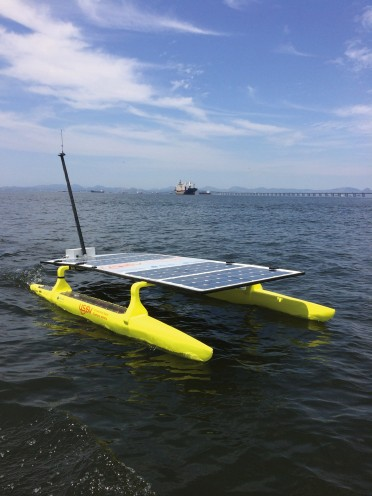
\includegraphics[scale=0.5]{figuras/barcoINTRODUCAO}
	\caption{Barco Autônomo Holos Brasil}
	\label{barcoINTRODUCAO}
\end{figure}
\section{Justificativa}

A  utilização de barcos elétricos que navegam e coletam dados de forma autônoma, sem piloto a bordo, já vem sendo difundida em projetos ao redor do mundo e hoje é tida como alternativa lógica a navegação comum. Este tipo de navegação normalmente é feito e controlado por uma pessoa em terra através de um computador ou dispositivo portátil. Com este intuito foi criado o barco autônomo, movido por energia solar, pela empresa Holos Brasil, que está situada no Rio de Janeiro. 
Este barco pode levar instrumentos para vários tipos de missão, tais como coleta de dados meteorológicos, oceanográficos ou fluviais (profundidade, traçado da topografia do leito) e para o estudo da vida aquática. 
Entretanto, esse barco além ser robusto e coleta diversas informações que não são referentes a qualidade da água e teve um custo muito alto, aproximadamente 300 mil reais.

Um barco que analise e colete, dados e água de forma automatizada, acarretaria em facilidade e praticidade para a ações de redução de poluentes e garantia de qualidade da água em pontos estratégicos encontrados em rios, lagos e reservatórios. Desta forma, este trabalho tem como intuito construir um Barco autônomo(Robarco).

O Robarco é uma embarcação inteligente controlada remotamente. Sua função é auxiliar na coleta e análise de água em pontos estratégicos de lagos, rios e reservatórios. A idéia do projeto surgiu da necessidade de se medir de forma autônoma, e obter dados em tempo real, sobre a qualidade da água em locais onde a logística demanda demasiadamente recursos financeiros e tempo. Dessa forma empresas poderiam utilizar recursos humanos menos especializados, poupar tempo e obter dados em intervalos de tempo menor. Além de evitar desastres ecológicos, evitarão possíveis multas e possíveis perdas de maquinário por corrosão entre outros danos causados pelo contato da água.

Este produto será projetado e criado por alunos de Engenharia Aerospacial, Engenharia Automotiva, Engenharia Eletrônica, Engenharia de Energia e Engenharia de Software da Universidade de Brasília (UnB), Faculdade do Gama (FGA).
%Fontes: http://revistapesquisa.fapesp.br/2017/03/17/barco-autonomo/
%http://www.eea.europa.eu/themes/water/water-pollution/overview


